\section{Online order assignment under the day-ahead plan}\label{sec:online}

The day-ahead plan fixes the capacities: $Q y_{ih}$ package-equivalents of scheduled lane capacity, $\pi w_i$ regular labour units, and an overtime allowance of $\rho\pi w_i$.
During the day, units arrive and must be assigned \emph{irrevocably}, without knowing the rest of the day.
This is the decision Amazon-style controllers take ``millions of times per hour''.
The recourse LP of \cref{sec:planning} evaluated on the realised demand is the \emph{hindsight} benchmark.
It is a lower bound on the cost of any non-anticipative policy that uses the same plan, because every online trajectory is a feasible solution of that LP.

\paragraph{Simulation model.}
The realised daily demand $\bfd$ (a draw from the true distribution) is split into 96 quarter-hour slots by a Dirichlet-perturbed intraday profile, with a night trough and lunch and evening peaks.
Within a slot, the batches $(j,k)$ arrive in random order.
Assigning one unit of $(j,k)$ to FC $i$ consumes one unit of $\mathrm{Inv}_{ik}$, $l_k$ labour units and $v_k$ package-equivalents of lane $(i,h(j))$.
Regular labour is consumed first, then overtime (at $c^{\mathrm{ot}}$, up to the cap); scheduled truck space is consumed first, then spot space (at $s_{ih}$).
The \emph{immediate} cost of a unit is therefore
\[
  \gamma_{ijk} = c^{\mathrm{fc}}_i + c^{\mathrm{lm}}_j + \lambda\ell_{ij}
   + c^{\mathrm{ot}} l_k\,\mathbb{1}[\text{regular labour at $i$ exhausted}]
   + s_{i,h(j)} v_k\,\mathbb{1}[\text{lane $(i,h(j))$ full}].
\]
A unit with no feasible FC (no inventory or no labour left anywhere it is stocked) is left unshipped at cost $p+\lambda$.
Batches are split exactly at the points where a resource changes cost regime, so the simulation is equivalent to unit-by-unit processing within a batch.

\paragraph{Policies.}
\begin{itemize}
  \item \textbf{Greedy}: $i^\star=\arg\min_i\gamma_{ijk}$. This is myopic: it depletes the cheap, on-time capacity near the early customers and leaves nothing for later ones.
  \item \textbf{Static bid prices} \citep{acimovic2015,talluri1998}: at the start of the day, solve the fluid LP, i.e.\ the recourse LP with the full capacities and the forecast demand $\hat\bfd$. Take the shadow prices $\mu\ge0$ of inventory, regular labour, overtime and lane capacity, and assign to
  \[ i^\star = \arg\min_i\ \gamma_{ijk} + \mu^{\mathrm{inv}}_{ik} + l_k\,\mu^{\mathrm{lab/ot}}_{i} + v_k\,\mu^{\mathrm{lane}}_{i,h(j)}, \]
  i.e.\ immediate cost plus the opportunity cost of the resources consumed. The labour price is the regular or the overtime one, whichever is currently being consumed; lane prices apply while scheduled space remains.
  \item \textbf{Re-solved bid prices}: the fluid LP is re-solved every hour with the \emph{remaining} capacities and the \emph{remaining} expected demand. The latter is the forecast times the remaining share of the intraday profile, scaled by an online learning factor per category, $(\text{observed} + a)/(\text{expected so far} + a)$ with $a=2000$ units of shrinkage.
  \item \textbf{Fluid LP tracking}: with the same hourly re-solves, the units of a batch are split across FCs in proportion to the LP flows $x^\star_{ijk}$, with a greedy fallback when a target FC has run out. This is the fluid-tracking idea behind probabilistic and correlated-rounding schemes \citep{jasin2015}.
  \item \textbf{Hindsight}: the clairvoyant LP (lower bound).
\end{itemize}
The online experiment uses the day-ahead plans of the proposed pipeline (SP with LightGBM + copula scenarios) on all 31 test days.
It runs 4 demand/arrival replications per day, i.e.\ 124 simulated days per policy, and the policies see the same arrivals (common random numbers).

\paragraph{Results.}
\begin{table}[t]
\centering\small
\caption{Online assignment over 124 simulated days (31 test days $\times$ 4 replications) under the day-ahead SP plan. Regret is the recourse cost above the clairvoyant hindsight LP; ``gap closed'' is the share of greedy's regret removed. Spot and overtime are daily means.}\label{tab:online}
\resizebox{\linewidth}{!}{\begin{tabular}{@{}lrrrrrrrrr@{}}\toprule
Policy & Recourse cost & Regret & s.e. & Gap closed & On-time & Unmet & Spot & Overtime & LPs \\
 & \EUR{}/day & \% & & \% & \% & \% & pkg-eq & labour u. & \\ \midrule
Greedy & 2{,}300{,}479 & 7.10 & 0.41 & 0 & 87.52 & 1.08 & 146{,}666 & 54{,}897 & 0 \\
Bid price (static) & 2{,}273{,}493 & 5.56 & 0.46 & 22 & 88.42 & 1.07 & 123{,}145 & 58{,}348 & 1 \\
Bid price (re-solve) & 2{,}205{,}156 & 2.35 & 0.45 & 67 & 90.37 & 0.89 & 77{,}349 & 48{,}941 & 24 \\
Fluid LP tracking & 2{,}190{,}863 & 1.53 & 0.48 & 79 & 90.94 & 0.91 & 64{,}586 & 48{,}982 & 24 \\
Hindsight LP & 2{,}116{,}083 & 0.00 & 0.00 & 100 & 91.54 & 0.61 & 47{,}906 & 46{,}302 & 1 \\
\bottomrule\end{tabular}
}
\end{table}

\begin{figure}[t]
  \centering
  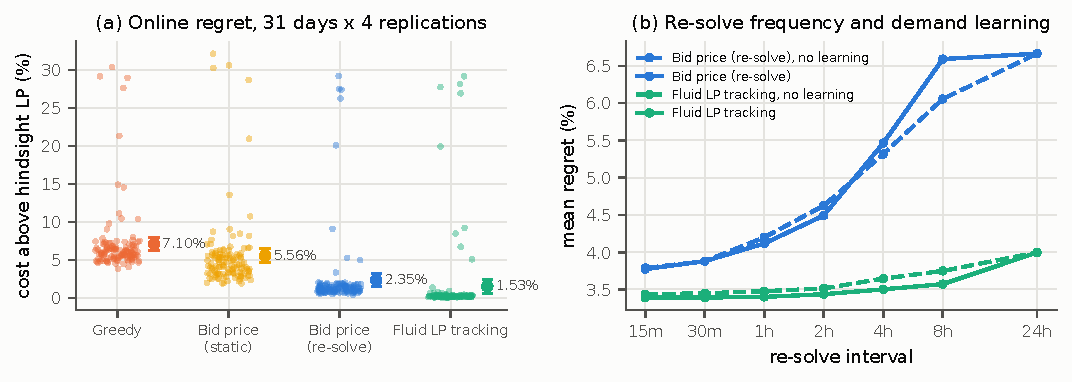
\includegraphics[width=\linewidth]{online}
  \caption{(a) Regret per simulated day; the outliers above 15\% are event days whose demand deviates strongly from the forecast. (b) Mean regret as a function of the re-solve interval, with and without online demand learning (every third test day). LP tracking is far less sensitive to stale information than bid prices.}
  \label{fig:online}
\end{figure}

\Cref{tab:online} and \cref{fig:online} show a clear ranking.
\begin{itemize}
  \item \textbf{Greedy assignment costs 7.1\% more than hindsight}, about \EUR{184}k per day. Most of the loss comes from spot capacity (three times the hindsight volume) and late deliveries. Greedy fills the cheap next-day lanes with the first customers of the day; later customers in other regions then need spot trucks or late lanes.
  \item \textbf{Static bid prices close 22\% of this gap.} That is of the same order as the 36\% reported by \citet{acimovic2015} on industry data with a comparable dual-value heuristic. They fail when the day deviates from the forecast: on 18\% of the days they are worse than greedy.
  \item \textbf{Re-solving hourly closes 67\%}, and \textbf{fluid LP tracking closes 79\%} (regret 1.5\%; 0.3\% on regular days). The policies are separated by \EUR{110}k per day between greedy and LP tracking.
  \item \textbf{Robustness.} Panel (b) explains the difference between the two LP-based policies. Bid prices are \emph{marginal} information: they are only valid locally, and degrade quickly as the state drifts from the one they were computed for (from 3.8\% regret at 15-minute re-solves to 6.7\% with a single solve). Tracking the LP \emph{flows} uses the full primal plan and is almost insensitive to the re-solve frequency (3.4\% to 4.0\%). Multiplicative demand learning brings only small gains, because the day-ahead forecast is already conditioned on yesterday's level.
  \item \textbf{Event days} remain the hardest, with 5.7\% regret even for LP tracking: the forecast error is large and arrives early in the day. This is where intraday re-forecasting and promise-date flexibility would pay most.
\end{itemize}
Computationally, all policies run a full day of about 25{,}000 batch decisions in under half a second, LP solves included. The LP is the same warm-started recourse model used by the planner, re-optimised by dual simplex in milliseconds.

